\documentclass[bachelor, och, labwork]{shiza}

\usepackage{subfigure}
\usepackage{tikz,pgfplots}
\pgfplotsset{compat=1.5}
\usepackage{float}
\usepackage{pdfpages}

\usepackage{titlesec}
\setcounter{secnumdepth}{4}
\titleformat{\paragraph}
{\normalfont\normalsize}{\theparagraph}{1em}{}
\titlespacing*{\paragraph}
{35.5pt}{3.25ex plus 1ex minus .2ex}{1.5ex plus .2ex}

\titleformat{\paragraph}[block]
{\hspace{1.25cm}\normalfont}
{\theparagraph}{1ex}{}
\titlespacing{\paragraph}
{0cm}{2ex plus 1ex minus .2ex}{.4ex plus.2ex}

% --------------------------------------------------------------------------%

\usepackage{multirow}
\usepackage[T2A]{fontenc}
\usepackage[utf8]{inputenc}
\usepackage{graphicx}
\graphicspath{ {./images/} }
\usepackage{tempora}

\usepackage[sort,compress]{cite}
\usepackage{amsmath}
\usepackage{amssymb}
\usepackage{amsthm}
\usepackage{fancyvrb}
\usepackage{listings}
\usepackage{listingsutf8}
\usepackage{longtable}
\usepackage{array}
\usepackage[english,russian]{babel}

\usepackage[hidelinks]{hyperref}
\usepackage{url}

\usepackage{underscore}
\usepackage{setspace}
\usepackage{indentfirst} 
\usepackage{mathtools}
\usepackage{amsfonts}
\usepackage{enumitem}
\usepackage{tikz}
\usepackage{minted}

\newcommand{\eqdef}{\stackrel {\rm def}{=}}
\newcommand{\specialcell}[2][c]{%
\begin{tabular}[#1]{@{}c@{}}#2\end{tabular}}

\renewcommand\theFancyVerbLine{\small\arabic{FancyVerbLine}}


\begin{document}
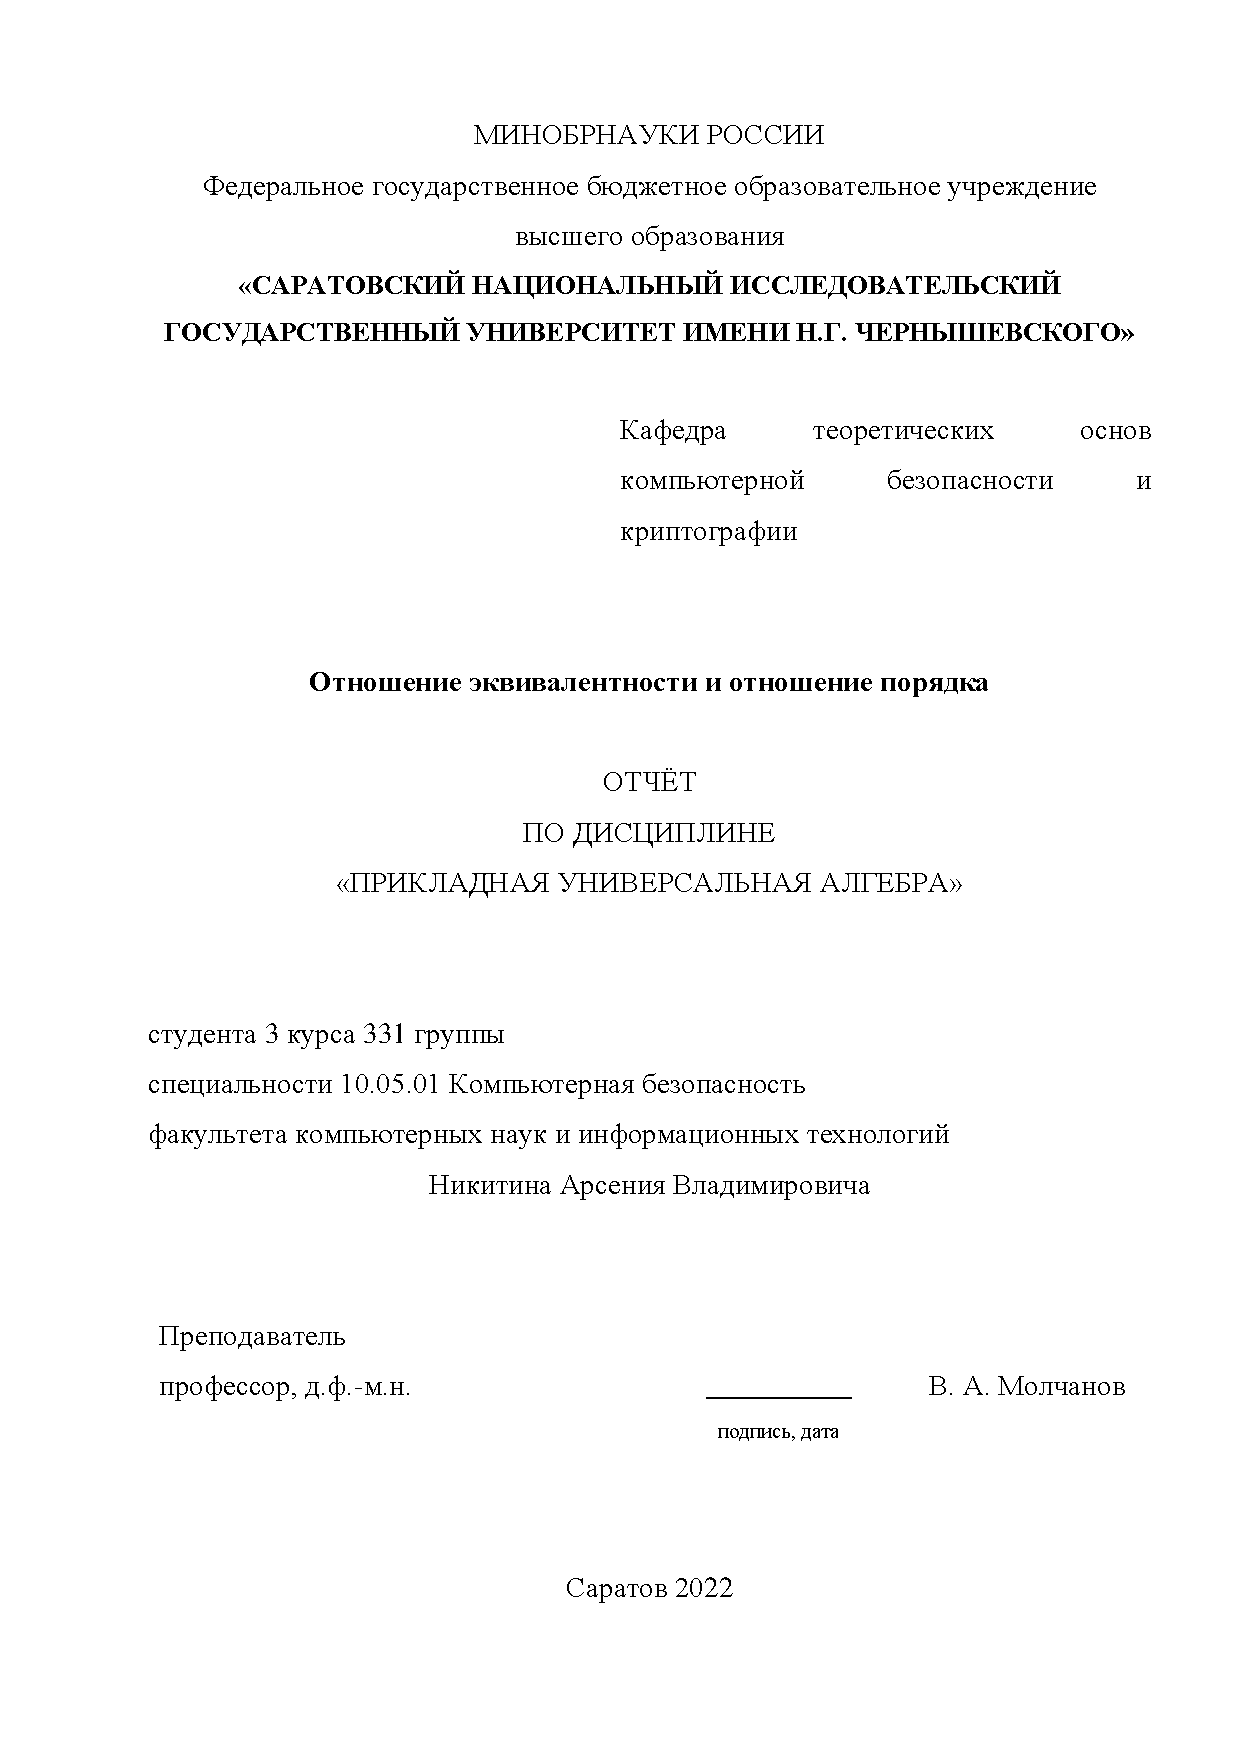
\includepdf{titul.pdf}

%-------------------------------------------------------------------------------

\tableofcontents

\intro

Бинарные отношения могут быть эквивалентными, и, поэтому на них могут строиться
фактор-множества. Если же бинарное отношение не является эквивалентностью, то
по определенному алгоритму можно построить эквивалентное замыкание данного
отношения. Также отношения могут обладать определенным порядком, в зависимости
от конкретных свойств. Если же отношение обладает порядком, то для данного
отношения можно построить диаграмму Хассе, а также для него могут быть
найдены минимальные и максимальные, и наименьшие и наибольшие элементы.
Также для бинарных отношений определены понятия контекста и концепта, а также
существует алгоритм вычисления решетки концептов.

\section{\textbf{Цель работы и порядок ее выполнения}}

\textbf{Цель работы} "--- изучение основных свойств бинарных отношений и 
операций замыкания бинарных отношений.

Порядок выполнения работы:

\begin{enumerate}

    \item Разобрать определения отношения эквивалентности, фактор-множества. 
    Разработать алгоритмы построения эквивалентного замыкания бинарного отношения 
    и системы представителей фактор-множества.  

    \item Разобрать определения отношения порядка и диаграммы Хассе. Разработать 
    алгоритмы вычисления минимальных (максимальных) и наименьших (наибольших) 
    элементов  и построения диаграммы Хассе. 

    \item Разобрать определения контекста и концепта. Разработать алгоритм 
    вычисления решетки концептов.

\end{enumerate}

\section{Теоретические сведения}

\subsection{Эквивалентное замыкание бинарного отношения}

\subsubsection{Определение эквивалентного замыкания отношения}

\textbf{Замыканием отношения} $R$ относительно свойства $P$ называется такое
множество $R^*$, что:

\begin{enumerate}
    \item $R \subset R^*$.
    \item $R^*$ Обладает свойством $P$.
    \item $R^*$ является подмножеством любого другого отношения, содержащего $R$
    и обладающего свойством $P$. 

    То есть $R^*$ является минимальным надмножеством множества $R$, 
    выдерживается $P$.
\end{enumerate}

Итак, исходя из вышесказанного, можно сделать вывод, что существуют 4 вида 
замыканий отношений: \textbf{транзитивное, симметричное, рефлексивное и
эквивалентное}.

На множестве $P(A^2)$ всех бинарных отношений между элементами множества $A$ 
следующие отображения являются операторами замыканий:
\begin{enumerate}
    \item $f_r(\rho) = \rho ~\cup \vartriangle_A$ -- наименьшее рефлексивное
    бинарное отношение, содержащее отношение $\rho \subset A^2$. 
    \item $f_s(\rho) = \rho \cup \rho^{-1}$ -- наименьшее симметричное
    бинарное отношение, содержащее отношение $\rho \subset A^2$.
    \item $f_t(\rho) = \cup^{\infty}_{n=1} \rho^n$ -- наименьшее транзитивное
    бинарное отношение, содержащее отношение $\rho \subset A^2$.
    \item $f_{eq}(\rho) = f_tf_sf_r(\rho)$ -- наименьшее отношение эквивалентности,
    содержащее отношение $\rho \subset A^2$.
\end{enumerate}

\subsubsection{Алгоритм построения эквивалентного замыкания бинарного отношения}

\textit{Вход.} Матрица $M(\rho)$ бинарного отношения $\rho$ размерности
$N \times N$.

\textit{Выход.} Эквивалентное замыкание бинарного отношения.

\begin{enumerate}
    \item Создать пустой список для хранения пар замыкания.
    \begin{enumerate}[label=a)]
        \item Цикл по $i ~\text{от}~ 1 ~\text{до}~ N$.
        \begin{enumerate}[label=1.]\item Если $M_{ii} = 0$, пару $(i, i)$ добавить в замыкание.\end{enumerate} 
    \end{enumerate}

    \begin{enumerate}[label=b)]
        \item Цикл по $i ~\text{от}~ 1 ~\text{до}~ N$, цикл по $j ~\text{от}~ 1 ~\text{до}~ N$.
        \begin{enumerate}[label=1.]\item Если $M_{ij} = 1 ~\text{и}~ M_{ji} = 0$, добавить пару $(j, i)$
        в замыкание.\end{enumerate}        
    \end{enumerate}

    \begin{enumerate}[label=c)]
        \item Цикл по $e ~\text{от}~ 1 ~\text{до}~ N$, цикл по $k ~\text{от}~ 1 ~\text{до}~ N$, 
        цикл по $i ~\text{от}~ 1 ~\text{до}~ N$, цикл по $j ~\text{от}~ 1 ~\text{до}~ N$.
        \begin{enumerate}[label=1.]\item Если $M_{ki}=M_{i,j}=1 ~\text{и}~ M_{ki}=0$, то добавить пару
        $(k, k)$ в замыкание транзитивности и замыкание эквивалентности.\end{enumerate}
    \end{enumerate}
    \item Ответ --- эквивалентное замыкание бинарного отношения $\rho$.
\end{enumerate}
Трудоемкость алгоритма $O(N+N^2+N^4)=O(N^4)$

\subsection{Фактор-множество отношения}

\subsubsection{Определение среза отношения через элемент}
Для любого подмножества $X \subset A$ множество:
\begin{center} $\rho(X)=\{b \in B:(x,b)\in \rho ~\text{для некоторого}~ X\}$ \end{center}
называется \textit{образом} множества $X$ относительно отношения $\rho$.

Образ одноэлементного множества $X=\{a\}$ относительно отношения $\rho$
обозначается символом $\rho(a)$ и называется также образом элемента $a$ или
\textit{срезом} отношения $\rho$ через элемент $a$.

\subsubsection{Определение фактор-множества отношения}

Эквивалентное бинарное отношение на множестве $A$ также принято обозначать как
$\varepsilon$.

Срезы $\varepsilon(a)$ называются \textit{классами эквивалентности} по отношению
$\varepsilon$ и сокращенно обозначаются символом [$a$].

Множество всех таких классов эквивалентности $\{[a]:a\in A\}$ называется 
\textit{фактор-множеством} множества $A$ по эквивалентности $\varepsilon$ и 
обозначается $A/\varepsilon$.

\subsubsection{Алгоритм построения фактор-множества бинарного отношения}

\textit{Вход.} Матрица $M(\rho)$ эквивалентного бинарного отношения $\rho$ размерности
$N \times N$.

\textit{Выход.} Фактор-множество отношения.

\begin{enumerate}
    \item Создать $N$ пустых списков.
    \begin{enumerate}[label=a)]
        \item Цикл по $i ~\text{от}~ 1 ~\text{до}~ N$, цикл по $j ~\text{от}~ 1 ~\text{до}~ N$.
        \begin{enumerate}[label=1.]\item Если $M_{ij} = 1$ добавить $j$ в список
        с номером $i$.\end{enumerate}        
    \end{enumerate}
    \item Ответ --- фактор-множество отношения.
\end{enumerate}
Трудоемкость алгоритма $O(N^2)$

\section{Программная реализация рассмотренных алгоритмов}
    
    \subsection{Результаты тестирования программы}

        \begin{figure}[H]
            \centering
            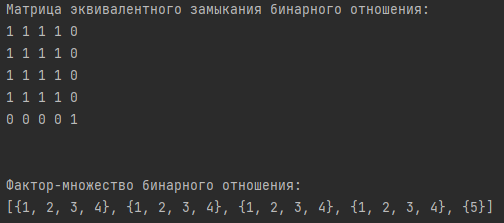
\includegraphics[width=0.8\textwidth]{pic/lab2.png}
            \caption{}
        \end{figure}
    
    \subsection{Код программы, реализующей рассмотренные алгоритмы}
    
        \inputminted[linenos,breaklines=true, fontsize=\small, style=bw]{python}{code/lab2.py}


\conclusion
В ходе лабораторной работы были рассмотрены понятия эквивалентного замыкания
бинарного отношения и получения представителей фактор-множества. Также были
получены алгоритмы вычисления минимальных и максимальных, и наименьших и наибольших
элементов бинарного отношения, а также был определен и программно реализован
алгоритм построения диаграммы Хассе. Был описан алгоритм построения решетки
концептов. Для всех алгоритмов произведена асимптотическая оценка.
\end{document}